\documentclass[12pt]{article}
\usepackage{geometry}                % See geometry.pdf to learn the layout options. There are lots.
\geometry{letterpaper}                   % ... or a4paper or a5paper or ...
%\geometry{landscape}                % Activate for for rotated page geometry
%\usepackage[parfill]{parskip}    % Activate to begin paragraphs with an empty line rather than an indent
\usepackage{graphicx}
\usepackage{amssymb}
\usepackage{amsmath}
\usepackage{epstopdf}
\usepackage{wrapfig}
\usepackage{natbib}
%\usepackage[square,comma,numbers,sort]{natbib}
\usepackage[pdftex, plainpages=false, colorlinks=true, linkcolor=blue, citecolor=blue, bookmarks=false]{hyperref}
\usepackage{setspace}
\usepackage{multicol}
\usepackage{sectsty}
\usepackage{url}
\usepackage{lipsum}
\usepackage{times}
\usepackage[tiny,compact]{titlesec}
\usepackage{fancyhdr}
\usepackage{deluxetable}
\usepackage[font=footnotesize,labelfont=bf]{caption}
\usepackage{verbatim}
\usepackage{acronym}

\setlength{\textwidth}{6.5in}
\setlength{\oddsidemargin}{0.0cm}
\setlength{\evensidemargin}{0.0cm}
\setlength{\topmargin}{-0.5in}
\setlength{\headheight}{0.2in}
\setlength{\headsep}{0.2in}
\setlength{\textheight}{9.in}
%\setlength{\footskip}{-0.2in}
%\setlength{\voffset}{0.0in}

\sectionfont{\normalsize}
\subsectionfont{\normalsize}
\subsubsectionfont{\normalsize}
\singlespacing

\input ../macros.tex
\input ../journal_abbr.tex

\pagestyle{fancy}
\fancyhf{}
\lhead{\fancyplain{}{\doctitle}}
\rhead{\fancyplain{}{S.M. Couch}}
\rfoot{\fancyplain{}{\thepage}}

\bibliographystyle{aasjournal}
%\bibliographystyle{hapj}
%\bibliographystyle{physrev}



%\titlespacing*{\section}{0in}{0.2in}{0in}
%\titlespacing*{\subsection}{0in}{0.1in}{0in}
\titleformat*{\subsection}{\itshape}
%\titlespacing*{\subsubsection}{0in}{0.in}{0in}
\titleformat*{\subsubsection}{\itshape}
\setlength{\abovecaptionskip}{3pt}

\begin{document}

\begin{center}
  {\bf \large Year 3 - CY2020 Allocation Renewal} \vspace{-0.1in}
\end{center}

\section{Project Achievements in Years 1 and 2}

\subsection{Significant Accomplishments and Progress on Project Milestones}

\subsubsection{3D simulations of magnetorotational core-collapse supernovae}

One of the key objectives for Year 1 of our INCITE project was to execute a parameter study of magnetorotational core-collapse supernova (CCSN) simulations using high-fidelity neutrino transport and magnetohydrodynamics (MHD) as implemented in our \sparkmone application, built in the \flash simulation framework \citep{Fryxell:2000, Dubey:2009}.
\sparkmone utilizes the new \spark high-order MHD solver \citep{couch:2017}, the M1 two-moment explicit neutrino transport method \citep{Shibata:2011a, oconnor:2015, oconnor:2018}, an accurate and efficient multipole gravity solver \citep{couch:2013c} including the general relativistic monopole correction \citep{Marek:2006}, and the \flash framework for adaptive mesh refinement (AMR), I/O, and runtime management.
The methods and physics included in \sparkmone make it one of the most high-fidelity and high-performance CCSN simulation tools in the world.

% \begin{figure*}[b!]
%   \begin{tabular}{ccc}
%     \includegraphics[width=2in]{fig_vr_m15u_3d_mag_annotated_0677.png} &
%     \includegraphics[width=2in]{fig_vr_m15u_3d_mag_rot_annotated_0695.png} &
%     \includegraphics[width=2in]{./fig_vr_m15u_3d_rot2_annotated_0696.png}    
%   \end{tabular}
%   \caption{Volume renderings of entropy from three of the 3D magnetorotational CCSN simulations that we are currently running on \mira as part of this INCITE project. Shown are cases with magnetic fields (left), magnetic fields and rotation (middle), and no magnetic fields but fast rotation (right). All of these simulations are currently at around 100 ms post-bounce and are on-going.} 
%   \label{f.m15u}
% \end{figure*}

\begin{figure*}[b!]
    \begin{tabular}{ccc}
        \includegraphics[width=2in]{m15u_3d_entr_slice_1126.png}&
        \includegraphics[width=2in]{m15u_3d_rot_entr_slice_1015.png}&
        \includegraphics[width=2in]{m15u_3d_mag_rot_entr_slice_1136.png}        
    \end{tabular}
    \caption{Slice plots of entropy from three of the 3D magnetorotational CCSN simulations that we ran on \mira as part of this INCITE project. Shown are cases with no magnetic fields or rotation (left), rotation but no magnetic fields (middle), and rotating and magnetic (right). In this plots, all simulations are currently at around 250 ms post-bounce.}
    \label{f.m15u}
\end{figure*}

The \spark MHD solver \citep{couch:2019a} implements the cell-centered method of generalized Lagrangian multipliers \citep[GLM;][]{Dedner:2002, Mignone:2010} to control the growth of the divergence of the magnetic field. 
The GLM-MHD scheme employs hyperbolic advection and parabolic damping of divergence errors in order to avoid expensive elliptic divergence cleaning \citep[e.g.,][]{Jiang:1999} or complicated staggered-mesh constrained transport \citep[e.g.,][]{Gardiner:2005, Lee:2009a, Lee:2013}.
\spark implements the GLM-MHD scheme via a finite-volume approach using high-order primitive reconstruction, multiple Riemann solvers for flux calculation, and method-of-lines time integration using multi-stage strong stability preserving (SSP) low-storage Runge-Kutta (RK) integrators of second- and third-order \citep[e.g.,][]{Gottlieb:1998}.
For realistic, non-Gamma-law equations of state, \spark avoids the approach of \citet{Colella:1985} used in other \flash solvers and adopts the volumetric internal energy, $\rho e$, as an auxiliary thermodynamic primitive variable instead, as in \citet{Almgren:2010}.
We have found this approach to be generally more robust but either method should be technically equivalent \citep[e.g.,][]{Zingale:2015}.
For our CCSN application, we use fifth-order WENO reconstruction \citep{Borges:2008}, second-order time integration, and the HLLC approximate Riemann solver \citep{toro:2009}.



Neutrino transport in \sparkmone is carried out using the M1 two-moment explicit approach described in \citet{oconnor:2015, oconnor:2018, oconnor:2018b}. 
The M1 scheme solves the first two angular moments of the Boltzmann equation for neutrinos and utilizes an analytic closure for the higher-order moments.
The neutrino fluxes, both in real space and in energy space, are computed explicitly as a hyperbolic system resulting in favorable performance and scaling properties (at the cost of time step sizes limited by the speed of light) while the matter-radiation source terms are computed implicitly.
This implicit solve is completely local and requires solving only a 4x4 matrix.
Our M1 solver is fully velocity-dependent, except in the calculation of the explicit flux terms, which is done to $\mathcal{O}(v/c)$.
In Year 1, we did not include inelastic neutrino scattering in the multidimensional version of our transport solver but during Year 2 we have successfully implemented and optimized this capability and will use it in the production simulations planned for Year 3.

The two-moment M1 approach is inherently more accurate than zeroth-moment only approaches such as flux-limited diffusion \citep[e.g.,][]{bruenn:2013, Dolence:2015, Lentz:2015}. 
M1 does not require a flux-limiter-based closure for the radiation fluxes as they are solved for directly.
Furthermore, the analytic closure we currently use for the moments beyond the first is simple and straightforward yet shows encouraging agreement with 1D Boltzmann and Monte Carlo neutrino transport calculations \citep{oconnor:2015, Murchikova:2017}.
As compared with flux-limited diffusion, M1 does not suffer from the inability to capture ``shadows'' inherent to FLD schemes.
A known limitation of M1 is cases in which distinct beams of radiation intersect, causing radiation ``shocks.''
The M1 solution in such cases becomes highly diffuse at the intersection.
This is a problem in, e.g., radiation hydrodynamic calculations of accretion disks or neutron star mergers.
For CCSNe, however, the radiation field is highly forward peaked and cases in which distinct beams of radiation might cross are essentially non-existent.
Hence, M1 is {\it ideally} suited for the CCSN problem due to its accuracy (for the specific problem) and efficiency.
In addition, the severe limitation of time steps determined by the speed of light is not so drastic in CCSNe since the explicit time step is already just a factor of a few larger than this thanks to the enormous sound speeds in the proto-neutron star (PNS).
Another significant advantage of M1 is that it is a fully multidimensional transport scheme, i.e., the solution at a given grid point is dependent on the fluxes from every direction around that point.
This is distinct from the often-adopted ``ray-by-ray'' approximation \citep[e.g.,][]{bruenn:2013, bruenn:2016, muller:2012a, Hanke:2013, Melson:2015, Lentz:2015} in which the transport problem is solved only along discrete radial rays.
The advantages of M1 for neutrino transport in CCSNe have not gone unnoticed and a number of groups are now adopting this approach \citep{Just:2015, Kuroda:2016, Skinner:2016, Roberts:2016, vartanyan:2018, vartanyan:2019}.


In our \flash CCSN application we have assumed that the composition of the matter throughout the entire computational domain is determined by nuclear statistical equilibrium (NSE).
This common approximation \citep[e.g.,][]{burrows:2007, Ott:2008, Dolence:2015, Skinner:2016, Roberts:2016, Kuroda:2016} is appropriate at high densities and temperatures where the nuclear reaction rates are sufficiently fast to establish equilibrium essentially instantly but becomes increasingly incorrect at low densities such as those in the silicon and oxygen shells surrounding the collapsing iron core.
Critically, correctly predicting the explosion energy or nucleosynthetic products such as radioactive nickel can be severely impacted by the inappropriate assumption of NSE \citep{bruenn:2016}.
\citet{bruenn:2016} advocate the use of an approximate nuclear network in regions that are not in NSE, while other groups \citep[e.g.,][]{muller:2012a, Melson:2015} use a ``flashing'' approach rather than a full network calculation.
We have recently implemented a method for transitioning to a nuclear network and appropriate EOS at low densities.
Our new approach blends the pressures between the high- and low-density EOS's to prevent spurious pressure discontinuities and uses an auxiliary variable to track whether a zone is entering or exiting NSE, allowing us to appropriately set the composition in the transition region.
This new capability will be included in Year 3 production simulations.

In Year 1, we successfully executed a parameter study of magnetorotational CCSN simulations. 
Figure \ref{f.m15u} shows volume renderings of entropy from three of the five high-resolution 3D simulations we ran on \mira and \thet. 
We opted to use the 15-\msun progenitor from \citet{heger:2005} in order to facilitate a direct comparison to the recent results of \citet{summa:2018}.
We ran five different cases for this one progenitor: (1) non-rotating, non-magnetic; (2) rotating, non-magnetic; (3) non-rotating, magnetic; (4) rotating, magnetic; and (5) rapidly rotating, non-magnetic. 
For rotating cases, we take the rotation profile directly from the progenitor model that was evolved with rotation and magnetic fields and prescriptions for angular momentum transport \citep{heger:2005}. 
For the rapidly-rotating case, we simply multiply the angular speed of the profile by two, making the rate of rotation similar to one of the models explored by \citet{summa:2018}.
The magnetic field is initialized with a quasi-poloidal field geometry with the peak strength set to match the field strength of the original progenitor model, about $10^8$ G. 
The peak angular speed of this model is about 0.2 rad s$^{-1}$ (0.4 rad s$^{-1}$ for the ``rapidly'' rotating case). 
This is, in fact, not very rapid rotation or field strength and so in these models we do not expect to see dramatic, magnetorotationally-dominated dynamics. 
Rather, we explored the impact of plausibly typical rotation rates and field strengths on the CCSN mechanism. 

% The 3D magnetorotational CCSN simulations are on-going and we fully expect to reach our target final simulation times by the end of Year 1. 
% Already, we are seeing an impact of rotation and, to a lesser extent, magnetic fields.
% We are already seeing that the rotating cases are closer to explosion.
% The presence of magnetic fields is, so far, having little impact on the gross dynamics of the simulations, but for these initial field strengths it will take a longer period of evolution to build of substantial field strengths. 
\begin{wrapfigure}[22]{l}{3in}
    \includegraphics[width=2.9in]{./fig_gradp_m25_o110_b9_0566.png}
    \caption{Equatorial slice plot of the gradient of pressure from a 3D magnetorotational CCSN simulation run as part of our previous INCITE project. The development of a non-axisymmetric rotational instabity in the PNS leads to the generation of strong spiral pressures waves. The gravitational wave emission is also significantly amplified.}
    \label{f.gradp}
\end{wrapfigure}
Our results from Year 1 simulations indicate that the presence of rotation, in particular, is helpful to CCSN shock revival \citep[e.g.,][]{summa:2018}. 
As shown in \ref{f.m15u}, the addition of rotation substantially increases the mean shock radius at the same time post-bounce. 
For the non-rotating, non-magnetic case (left panel), the shock is already receding by this point whereas for all cases including rotation the shock remains stalled at large radii ($\sim$200 km).
The right panel of Figure \ref{f.m15u} shows the case including both realistic rotation and weak initial magnetic fields.
The magnetic fields, even if weak, may still have an impact on the behavior of the turbulence in the gain region and the PNS.
Indeed, we see that while the field strengths, even at this point post-bounce, are not dynamically strong, there is still a noticeable impact on the overall evolution of the simulation. 
The shock is at slightly larger radii than the rotating-only case and the entropies in the gain layer are on average greater. 
This simulation is closer to explosion than the comparable case without magnetic fields. 
Detailed analysis and comparisons are underway now.
This anallysis will include exploring the presence of a non-axisymmetric rotational instability in the PNS \citep{wheeler:2007, ott:2005}. 
In work based on simulations ran as part of our previous INCITE allocation, we have identified the emergence of such an instability for magnetic and rotating initial conditions. 
This instability can generate strong pressure waves that transport energy to the gain region, and also leads to very loud gravitational wave signals.
An image of the strong pressure waves is shown in Figure \ref{f.gradp}.

\subsubsection{3D Simulations of CCSN Progenitors}

One of the most remarkable and exciting results of recent 3D simulations of the CCSN mechanism is the discovery that  realistic non-spherical structure in the progenitor star can have a dramatic impact \citep{couch:2013b, couch:2015, couch:2015a, muller:2015, muller:2017, oconnor:2018b}.
The breaking of spherical symmetry is manifest in the turbulent convection driven by nuclear burning in the cores of massive stars.
As a massive star nears collapse, strongly convective burning in the Si and O shells surrounding the iron core can reach speeds of nearly 1000 km s$^{-1}$ and is characteristically very large in spatial scale \citep{Arnett:2011, couch:2015a, muller:2016a}.
These convective perturbations will reach the stalled shock shortly after core bounce and can aid neutrino-driven explosions by either enhancing the strength of post-shock turbulence \citep{couch:2015} or causing large scale ``forced shock deformations'' \citep{muller:2017}, or both.
These results serve to remind us that CCSN mechanism simulations are initial value problems and that the details of our initial conditions matter tremendously!
Our work inaugurated the era of detailed investigation into the impact of 3D progenitor structure on the CCSN mechanism \citep{couch:2013b, couch:2015a}.
As part of this INCITE project we are advancing the investigation into 3D progenitor structure substantially.
Specifically, we are simulating 3D progenitors including rotation and magnetic fields.

\begin{wrapfigure}[21]{r}{3in}
  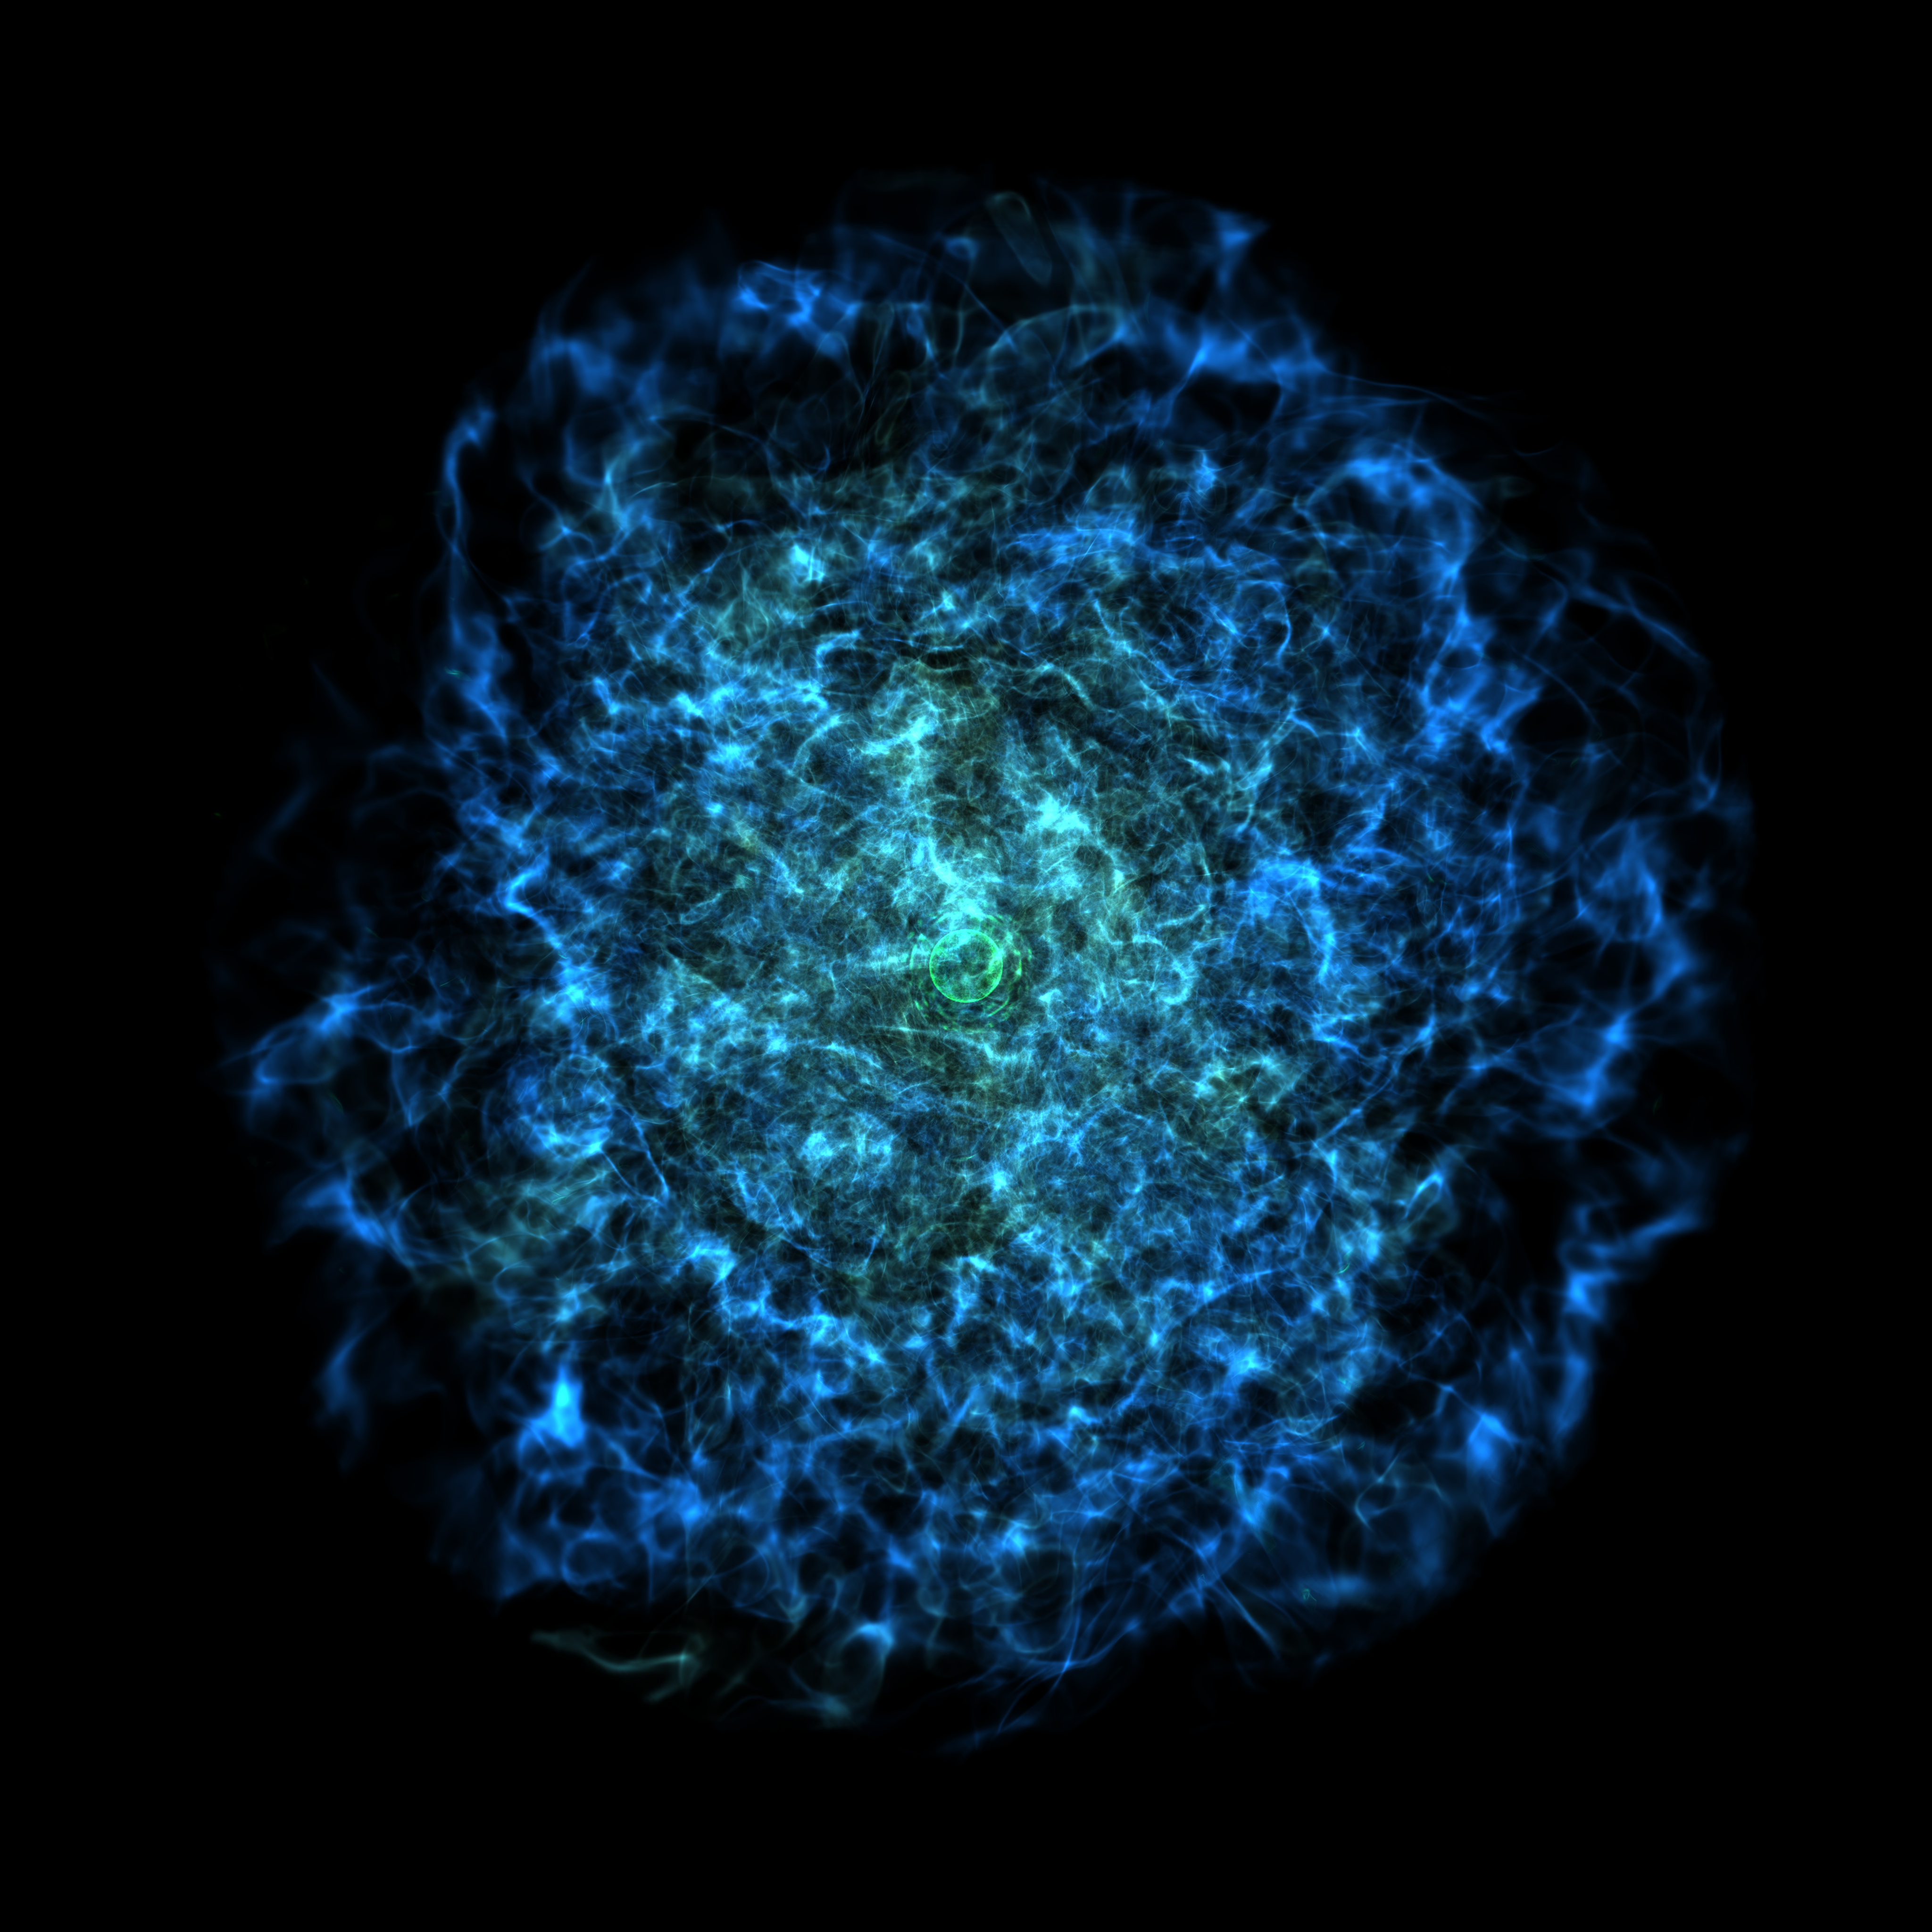
\includegraphics[width=2.9in]{mag_vel_face_on_no_rot_prog3d_oct_vol_0834.jpg}
  \caption{Volume rendering of the velocity magnitude from a 3D progenitor simulation run in full ``$4\pi$'' geometry during Years 1 and 2 of this project. Peak convective speeds reach over 300 km/s prior to core collapse. This simulation is being used as initial conditions for Year 2 CCSN simulations.}
  \label{f.progen}
\end{wrapfigure}
A key milestone for Years 1 and 2 was to carry out new, high-fidelity 3D simulations of the final minutes of stellar evolution to the point of iron core collapse.
%For these simulations we used the \spark MHD solver \citep{couch:2019a} and include rotation and magnetic fields {\it for the first time ever} in a 3D CCSN progenitor simulation.
We are used 1D massive star evolution models constructed using MESA \citep{paxton:2011, paxton:2013, paxton:2015}, initialized in 3D approximately five minutes prior to core collapse.
During Years 1 and 2 we ran a full-3D non-rotating, non-magnetic case all the way to the point of iron core collapse. 
In second half of Year 2 we will carry out a second full 3D model that includes both rotation and magnetic fields.
%In the original proposal, we planned four 3D progenitor simulations in Year 1.
Our test simulations executed showed that the expense of the simulations increases significantly as the stars approach collapse.
This is due to more vigorous nuclear burning in the core, increasing the expense of the nuclear network solve.
Therefore, in order to ensure that we can simulate sufficiently long time scales, we have opted to execute just these two simulations rather than the originally-planned four.


In Years 1 and 2, we made substantial gains in improving our simulation approach for 3D CCSN progenitors.
We improved the OpenMP threading of our nuclear network code. 
We improved the efficiency of the empirical load balancing approach our progenitor application uses. 
We tested several approaches to the initial mapping of the 1D progenitor model to the 3D domain and have improved our approach to stabilizes the initial conditions. 
We implemented new, modern reaction rates for electron captures and for key carbon reactions.
And, importantly, we have successfully, and efficiently, run a full production simulation all the way to core instability and collapse.

% We are now ready to begin our 3D progenitor production simulations on \mira. 
For the rotating, magnetic progenitor we are using a MESA model constructed using the magnetic field production and angular momentum transport model of \citet{spruit:2002}, as implemented for stellar evolution by \citet{heger:2005, paxton:2015}.
This model yields a realistic rotation profile and an estimate for the {\it strength} of the magnetic field as a function of radius in the star. 
There is very limited information about the 3D geometry of the field.
To address this, we are initializing the field in a random, divergenceless fashion with a typical strength matching the 1D MESA model estimate.
We will then allow the field to relax to a quasi-steady-state configuration.
This transition should occur on the rotational and convective time scale, both of which are about 30 s. 
We will simulate roughly 3 to 5 minutes of evolution up to core collapse.

\subsubsection{High-resolution Simulation of Magnetorotational Turbulence}

Our final simulation milestone for Year 1 was to execute a high-resolution simulation of magnetorotational turbulence in the CCSN gain region. 
For this simulation, we used the ``rapidly'' rotating conditions described above and allow for higher resolution in the gain layer using AMR.
This simulation required many more zones than the fiducial resolution case and was a standalone Capability-scale simulation.
This simulation was run until 100 ms post-bounce and we are now analyzing the results and comparing to the lower-resolution case. 

\subsubsection{Long time simulations of MHD CCSNe}

In Year 2 of this project we are carrying out the 3D simulations of magnetorotational CCSNe from Year 1 to late times, nearing one second post-bounce.
Long time scale simulations are crucial for accurately predicting the explosion energy, PNS mass, nucleosynthesis, etc. \citep{bruenn:2016, muller:2017}.
For any of the simulations that fail to explode, we will attempt to simulate late enough times to capture the onset of PNS collapse to a black hole.
This has the potential to elucidate some details of the formation of stellar mass black holes, such as those that have been detected by aLIGO \citep{abbott:2016, abbott:2017}.
We have recently shown \citep{pan:2018} that the GR effective potential approach can fairly accurately predict black hole formation time in 2D as compared to 1D fully GR simulations \citep{oconnor:2011}.

The nucleosynthetic yields from CCSN simulations are a key quantity that can be directly compared to observations and laboratory measurements of cosmic abundances.
We will compute the detailed nucleosynthesis from these late-time CCSN simulations.
This will be accomplished as a post-processing step using the open-source SkyNet nuclear reaction network code developed by Co-I Roberts.
The input for the nuclear reaction networks will be passive tracer particle data that records thermodynamic trajectory information from our \flash CCSN simulations.
\flash already includes a well-developed, efficient passive-particle framework that has been used extensively in the calculation of nucleosynthesis in Type Ia supernova simulations \citep[e.g.,][]{long:2014}.
We will compute detailed abundances for elements such as radioactive nickel and titanium, two key observable quantities, and we will also examine how rotation and magnetic fields can influence the conditions for very heavy element formation and the r-process.

% Each of the four 3D simulations will require 16M core-hours on \mira and 10 TB of online storage (see Section \ref{sec:performance}).
% Including 2M \mira core-hours for development and testing, the total request for this milestone is 66M \mira core-hours and 40 TB of online storage.

These simulations have been restarted from simulations carried over from Year 1 and are running in the Capability queue on {\it Mira}. Substantial progress has been made on these simulations and they are nearing completion.

\subsubsection{High-resolution simulation of MHD dynamos in the proto-neutron star}

There is a very strong shear layer at the edge of rotating PNS's that is unstable to the magnetorotational instability \citep[MRI,][]{akiyama:2003, burrows:2007}.
The presence of convection combined with rotation in the PNS can also lead to an $\alpha$-$\Omega$ dynamo \citep{mosta:2015}.
Both mechanisms can lead to exponential amplification of magnetic fields with dramatic implications for the CCSN mechanism.
Accurately capturing either process is extremely challenging computationally, requiring extremely high resolution to capture the fastest growing modes of these instabilities \citep{mosta:2015}.
In Year 2 of this project, we will carry out an extremely high resolution simulation of a rotating PNS in order to study the rapid growth of magnetic fields via the MRI and dynamo.
This simulation will go beyond \citet{mosta:2015} in a number of ways: we will use our M1 neutrino transport method rather than leakage, we will include the entire solid angle of the sphere rather than just a 90$^\circ$ wedge, and will simulate to later times in the aim of capturing the saturation of the magnetic fields.
Using AMR, we will add two extra levels of refinement beyond our fiducial resolution only in the shear layer surrounding the PNS, between 15\,km and 40\,km, bringing the finest resolution elements to 163\,m.
This approach was piloted for capturing turbulence in the gain region during our current INCITE project and will avoid adding additional zones in regions that are stable to the instabilities of interest.
This is not as high as the highest resolution used by \citet{mosta:2015} but we plan to go to much longer time scales, as much as 100 ms post-bounce.
This simulation will comprise about 100 million zones in 3D and require about 200,000 time steps to reach 100 ms.
%The expense for this simulation will be 60M core-hours on \mira and will require 40 TB of online storage. We request an additional 2M core-hours for testing and development.

So far in Year 2 we have analyzed simulations from Year 1 that will serves as the initial conditions for this high-resolution simulation. We anticipate starting this simulation in Q3 of Year 2. Given the extreme resolution of this simulation, it will run in the Capability queue from the outset.

\subsubsection{MHD simulation of CCSN progenitors} 

In Year 2, we are extending the Year 1 study of iron core collapse to rotating and magnetic stars.
We will simulate the final five minutes of stellar evolution to core collapse in 3D for a 25-\msun progenitor stars for both ``high'' and ``low'' core rotation rates.
As in Year 1, all final models will be made publicly available.
% Each such simulation will require 5M core-hours on \mira, for a total of 20M core-hours for the four simulations.
% We request 10 TB of online storage for these simulations.
% We request an additional 2M core-hours for testing and development.

These simulations will be started in Q3 of Year 2. We are now tuning our progenitor application to make better use of OpenMP threading and developing realistic initial conditions for the magnetic field strength and geometry.

\subsubsection{CCSN simulation with 3D progenitors}

In Year 2 we will use the 3D progenitor models generated in Year 1 for 3D CCSN simulations on \thet.
The progenitor model for these simulations is now finished and ready to be used in CCSN simulations. 
For these simulations, we will enhance the physical fidelity of our neutrino transport by incorporating our newly-implemented neutrino-electron scattering capability and the latest, most accurate electron capture rates. 

% For these four simulations we will use the 15-\msun 3D progenitor simulated during Years 1 and 2.
% For this milestone we request a total of 16M \thet core-hours (52M \mira-equivalent core-hours) and 20 TB of online storage.
% Plus an additional 2M \thet core-hours for development and testing, the total request for \thet in Y2 is 18M core-hours (58.5M \mira-equivalent core-hours).


% \subsubsection{Implement microphysics from TEAMS SciDAC collaboration and neutrino-electron scattering (NES)} 

% This planned open-source microphysics framework will incorporate the latest, state of the art neutrino interactions and cross sections that are fully self-consistent with the underlying EOS.

% Built on NuLib. Currently FLASH (and hence Spark-M1) is the only CCSN code in TEAMS that already utilizes NuLib, so we are good.

% The TEAMS microphysics package is not yet ready for production simulations. We have during Q1 finished an implementation of NES and are now testing it in 1D and 2D simulations. We anticipate being able to use this new capability in our planned 2019 CCSN simulations. 


\begin{figure*}
    \includegraphics[width=6in]{./gw_trains.png}
    \caption{Gravitational wave strains from the 3D simulations of \citet{oconnor:2018}, carried out under a prior INCITE award. Our work showed for the first time that the presence of 3D structure in the progenitor star leaves a detectable imprint on the gravitational wave emission.}
    \label{f.strains}
  \end{figure*}
  
  \subsubsection{Fundamentally 3D Phenomena in CCSNe}
  
  Recently, we submitted a publication detailing results based on simulations carried out under our previous INCITE award \citep{oconnor:2018b}.
  This work includes several full 3D, high-resolution simulations using our M1 neutrino transport in \flash, representing over 100 Million core-hours of work on \mira.
  In these simulations, we identify and analyze several essentially 3D aspects of CCSNe, including the presence of a new instability in the neutrino emission called the Lepton-number Emission Self-sustaining Asymmetry (LESA), first reported by \citep{tamborra:2014}. 
  We are the first group to confirm the presence of the LESA in CCSNe and, since we use a very different transport approach, our work strongly implies this is not a numerical artifact but a real physical instability. 
  
  In \citet{oconnor:2018}, we also show that the presence of the non-spherical, 3D progenitor structure has several important impacts on the CCSN mechanism. 
  We show that convective motion in the progenitor can substantially increase the proximity to explosion.
  We also showed that 3D structure in the progenitor can leave a measurable imprint on the gravitational wave emission from CCSNe that could be detected by, e.g., LIGO. 
  The gravitational wave strains from our simulations are shown in Figure \ref{f.strains}.
  
\subsection{Project Usage}

\begin{figure}
    \begin{tabular}{cc}
        \includegraphics[width=3.25in]{on_track_graph_mira_2018.png}
        \includegraphics[width=3.25in]{categorized_hours_graph_mira_2018.png} \\
        \includegraphics[width=3.25in]{on_track_graph_2018}
        \includegraphics[width=3.25in]{categorized_hours_graph_2018} 
    \end{tabular}
    \caption{Allocation usage in Year 1 on {\it Mira} and {\thet}.}
    \label{fig:usageY1}
\end{figure}
    
\begin{figure}
%   \begin{tabular}{cc}
    \includegraphics[width=3.25in]{on_track_graph_mira.png}
    \includegraphics[width=3.25in]{categorized_hours_graph_mira.png} \\
%     \includegraphics[width=3.25in]{on_track_graph}
%     \includegraphics[width=3.25in]{categorized_hours_graph} 
%   \end{tabular}
    \caption{Allocation usage in Year 2 on {\it Mira}.}
    \label{fig:usage}
\end{figure}
    
In Year 1 of our allocation, we fully expended our allocations on both \mira and \thet (see Figure \ref{fig:usageY1}). 
On \thet, despite a late start to our production simulations, we exceeded our initial allocation by 12\%. 

So far in 2019 we expended 66M core-hours on Mira out of our total 2019 allocation of 150M core-hours (44\% usage). 
This is just slightly behind the linear usage curve, though our burn rate in Q2 was substantially larger than for Q1.
We are now running one of our primary simulation milestones in the Capability queue and will start a second Capability-scale simulation in the next week or two. 
Figure \ref{fig:usage} we show our current usage and categorized hours on Mira.

We have yet to start running production simulations on Theta for two reasons. 
First, during Q1 we spent some effort continuing to tune our production application for Theta. 
This is largely complete now.
The second reason for the delayed start is that we were waiting on the completion of 3D supernovae progenitor simulations that we had planned to use as the initial conditions for our simulations on Theta this year.
These simulations are now complete and a paper is in preparation describing them. 
We are now prepared to start these simulations during Q3. 
Based on our experience last year running on Theta, we do not anticipate any difficulty in expending our entire allocation before the end of the calendar year.
       
    

% \begin{figure}
%   \begin{tabular}{cc} 
%     \includegraphics[width=6.5in]{fig_theta_scaling_j4.pdf}
%   \end{tabular}
%   \caption{Weak scaling test on Theta. Different colors represent different combinations of MPI and OpenMP tasks. }
%   \label{fig:theta}
% \end{figure}


\subsection{Application Parallel Performance}

\begin{wrapfigure}[15]{l}{3in}
    \includegraphics[width=3in]{wkScaleSparkAll.pdf} 
    \caption{Weak scaling parallel efficiency of our \sparkmone application on \thet.}   
    \label{f.wkScaleThet}
\end{wrapfigure}

As shown in our original proposal, our application demonstrates good parallel performance. 
In Figure \ref{f.wkScaleThet} we show the weak scaling parallel efficiency of \sparkmone on \thet for up to 2048 nodes. 
At production scales ($\gtrsim128$ nodes), we see an efficiency of around 80\%. 
Considering the immense communication requirements of our M1 transport solver, we consider this good performance. 

We have also substantially improved our overall appliation performance on \thet during Years 1 and 2. 
At the time of our original proposal, \sparkmone on \thet and a performance metric of 91 mega-zone-updates per node-hour. 
We have optimized the single-node performance of our application to better utilize KNL hardware threads, high-bandwidth memory, and OpenMP parallelism. 
For the same application we now achieve a metric of 132 mega-zone-updates per node-hour, and increase in single-node performance of 44\%. 

% \section{Code Development}


% We planned two code development milestones for Year 1: implement a ``marching cubes'' approach for our EOS and opacity tables and develop a simulation workflow management tool in Python.
% Both efforts are still underway.
% While developing the marching cubes capability we found that we could significantly accelerate our table interpolations by reordering some of the large arrays.
% This allowed for efficient vectorization by the compiler and sped up our table interpolations, both EOS and opacity, by about a factor of two. 
% This improvement makes these aspects of our simulations relatively cheap, although the memory cost of the large tables is still high.
% Nevertheless, we have downgraded the priority of implementing the marching cubes approach.\footnote{Never let optimization slow you down.}
% We will still complete this implementation as person-power allows.

% We have continued to develop workflow  tools for managing our large simulations on \mira and \thet. 
% We have implemented new {\tt bash} scripts that automatically configure and submit restart jobs, which will substantially increase our queue throughput. 
% We are incorporating these new tools into our existing Python tool chain.
% We have also developed Python code to automatically configure and setup simulation parameter studies and generate job submission scripts. 
% Work on this tool continues and we will implement functionality for some limited runtime visualization and automatic data archiving in the near future.

We have also made significant progress on other code development relevant to, but not directly planned as part of, this INCITE program. 
In our neutrino transport, we have implemented neutrino-electron inelastic scattering, an important process that we have so far only included during the 1D collapse phase of our simulations. 
We have also begun porting our \spark MHD solver to the DOE Exascale Computing Project (ECP)-supported AMReX framework. 
We are doing this within the new version of \flash that is being developed as part of the DOE ECP. 
We anticipate moving to the AMReX version of \flash in the future for our production simulations.


% For Year 2, we continued to make improvements to our \sparkmone application.
% As originally proposed, we will implement the TEAMS SciDAC EOS and opacity framework. 
% In collaboration with researchers at the University of Washington and the University of Tennessee, Co-PI Roberts is now working on the initial implementation of this framework.
% This effort will enhance the physical fidelity of the EOS and neutrino opacities we use in our simulations. 

The second major code development effort we performed in Year 2 is the implementation of high-order, single-step methods for MHD in our CCSN application.
This is work also supported by the TEAMS SciDAC collaboration.
Chelsea Harris, a new research associate at MSU, is leading this effort. 
Our \spark MHD solver is written in such a way to make implementation of this new approach straight-forward. 
A high-order single-step method will both increase the accuracy of our simulations while also decreasing the overall communication burden. 
This as the potential to significantly improve our computational efficiency.
We will also continue porting our various physics routines, particularly \spark, to the AMReX-capable version of \flash.

\subsection{Data Storage}

At present, we have 280 TB of online storage on the \mira filesystem and approximately 200 TB on archival storage. 
At this stage, we are continually triaging our on-disk data and moving to tape as we are able to free up disk for new simulations.


\section{Project Plans for Year 3}

During Years 1 and 2 we have largely achieved our originally-planned goals for this three-year project.
Therefore, our goals for Year 3 will be largely unchanged except for minor course corrections based on the actual achievements of the first two years. 
One major change is necessitated by the delay of the \aurora system. 
We had originally proposed an extensive parameter study of 3D magnetorotational CCSNe on \aurora for Year 3.
We have opted to de-scope this study to far fewer simulations to be executed on \thet instead. 
This does require, however, a substantial increase in our request for \thet in Year 3. 
We had originally requested 500k node-hours on \thet in Year 3 but to achieve the goals we outline below we now request a total of 1M node-hours on \thet for 2020.

Based on our updated application performance studies on \thet, we estimate that for 500 ms of post-bounce evolution, our \sparkmone CCSN simulations will require approximately 100k node-hours when including neutrino-electron scattering.
This performance is very competitive with comparable state-of-the-art CCSN simulations on comparable hardware platforms \citep{vartanyan:2019}.

\subsection{MHD CCSN Simulations Using 3D Progenitors}
\label{sec:Y3mrccsn}

In Year 3 we will use the 3D progenitor models generated in Year 2 for 3D MHD CCSN simulations on \thet.
These progenitors will be simulated in 3D with both rotation and magnetic fields. 
We will carry out two new CCSN simulations, one from a fully magnetorotational progenitor and one in a rotating-only progenitor. 
As with all planned Year 3 simulations, we include our newly-implemented neutrino-electron scattering capability.
For this milestone we request a total of 250k node-hours and 40 TB of online storage.

\subsection{Late time 3D Simulations of Magnetorotational CCSNe from 3D Progenitors}
\label{sec:Y3late}

In Year 3 we will continue two CCSN simulations from 3D progenitors started in Year 2 to about one second post-bounce.
As in Year 2, we will study the explosion energies, PNS masses, nucleosynthesis, and black hole formation times in these simulations as appropriate.
For this milestone we request a total of 250k node-hours and 40 TB of online storage.


\subsection{Magnetorotational CCSN Parameter Study in 3D Progenitors}
\label{sec:Y3aurora}

The four 3D simulations planned above will be executed in progenitor models that have been evolved in 3D. 
At this point, those are the only such models we expect to be available, at least during the beginning of Year 3.
In order to augment this progenitor set, and further explore the impact of rotation and magnetic fields across the range of potential CCSN progenitors, we will run four additional 3D CCSN simulations in the 1D magnetorotational progenitor models of \citep{heger:2005}. 
These models include realistic rotation profiles and rough estimates of magnetic field strengths. 
In order to increase the realism of these models in the absence of fully 3D evolution to core collapse, we will add multidimensional perturbations in the convective shells of these models using the vector spherical harmonics formalism of \citet{chatzopoulos:2014}. 
Such an approach has been used in several recent studies \citep{oconnor:2018b, vartanyan:2019}.
We will select a range of progenitor compactnesses \citep{oconnor:2011, sukhbold:2018} in this study.
For these simulations, we will include inelastic neutrino scattering \citep{oconnor:2015, burrows:2016}.
Each simulation will cost about 100k node-hours to reach around 500 ms post-bounce. 
Thus, we request a total of 500k node-hours and 80 TB of online storage for this milestone.

\subsection{Code Development}

For the planned Year 3 milestones above we require no further code development. 
The only major relevant development effort we plan to undertake in Year 3 is to continue to adapt our \sparkmone application to the new AMReX-based FLASH5.
This version of FLASH is targeted at the exascale and is being supported by the DOE Exascale Computing Project.

\renewcommand\bibsection{\section*{References}}
\setlength{\bibsep}{2pt}
%\begin{multicols}{2}
\bibliography{AchievePlans}
%\end{multicols}




\end{document}
